% ============================================
% SPARROW AI - Technical Implementation Document
% For Hackathon Judges
% ============================================

\documentclass[11pt,a4paper]{article}

\usepackage[utf8]{inputenc}
\usepackage[T1]{fontenc}
\usepackage{lmodern}
\usepackage[margin=1in]{geometry}
\usepackage{graphicx}
\usepackage{booktabs}
\usepackage{array}
\usepackage{xcolor}
\usepackage{hyperref}
\usepackage{tikz}
\usepackage{enumitem}
\usepackage{fancyhdr}

% Colors
\definecolor{sparrowblue}{RGB}{37, 99, 235}
\definecolor{sparrowdark}{RGB}{15, 23, 42}
\definecolor{googleblue}{RGB}{66, 133, 244}
\definecolor{elevenlabspurple}{RGB}{138, 43, 226}

% Header/Footer
\pagestyle{fancy}
\fancyhf{}
\fancyhead[L]{\textcolor{sparrowblue}{\textbf{Sparrow AI}}}
\fancyhead[R]{\textcolor{gray}{Technical Implementation}}
\fancyfoot[C]{\thepage}

\hypersetup{
    colorlinks=true,
    linkcolor=sparrowblue,
    urlcolor=sparrowblue
}

\begin{document}

% -------------------- Title --------------------
\begin{center}
{\Huge\textbf{\textcolor{sparrowblue}{Sparrow AI}}}\\[0.5cm]
{\Large Technical Implementation Document}\\[0.3cm]
{\large AI Partner Catalyst Hackathon - ElevenLabs Challenge}\\[0.5cm]
\rule{12cm}{0.5pt}
\end{center}

\vspace{0.5cm}

% -------------------- Executive Summary --------------------
\section*{Executive Summary}

Sparrow AI is a voice-first sales training platform that combines \textbf{ElevenLabs Conversational AI} with \textbf{Google Gemini 2.0 Flash} to create realistic AI sales prospects. Users practice cold calls, discovery conversations, and objection handling through natural voice interactions, receiving instant AI-powered feedback.

\begin{center}
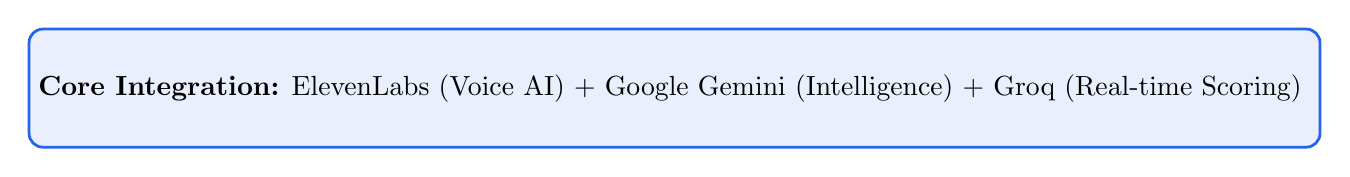
\begin{tikzpicture}
\node[draw=sparrowblue, line width=1pt, rounded corners=5pt, fill=sparrowblue!10, minimum width=14cm, minimum height=1.5cm, align=center] {
\textbf{Core Integration:} ElevenLabs (Voice AI) + Google Gemini (Intelligence) + Groq (Real-time Scoring)
};
\end{tikzpicture}
\end{center}

% -------------------- Architecture --------------------
\section{System Architecture}

\subsection{Technology Stack}

\begin{table}[h]
\centering
\begin{tabular}{lll}
\toprule
\textbf{Layer} & \textbf{Technology} & \textbf{Purpose}\\
\midrule
Voice AI & ElevenLabs Conversational AI & Real-time voice conversations\\
Intelligence & Google Gemini 2.0 Flash & Persona generation, call analysis\\
Fast Inference & Groq (Llama 3.1 70B) & Real-time scoring during calls\\
Frontend & Next.js 15 + React 19 & Modern web application\\
Database & Supabase (PostgreSQL) & Data persistence\\
Auth & Clerk & User authentication\\
Hosting & Vercel & Edge deployment\\
\bottomrule
\end{tabular}
\end{table}

\subsection{Data Flow}

\begin{enumerate}[leftmargin=*]
\item \textbf{Persona Generation}: User selects parameters $\rightarrow$ Gemini generates realistic prospect
\item \textbf{Voice Session}: ElevenLabs creates WebSocket connection with dynamic variables
\item \textbf{Conversation}: User speaks $\rightarrow$ ElevenLabs STT $\rightarrow$ LLM response $\rightarrow$ ElevenLabs TTS
\item \textbf{Analysis}: Call ends $\rightarrow$ Transcript sent to Gemini for detailed feedback
\item \textbf{Scoring}: Groq provides instant scores; Gemini provides deep analysis
\end{enumerate}

% -------------------- ElevenLabs Integration --------------------
\section{ElevenLabs Integration}

\subsection{Conversational AI Implementation}

We use the ElevenLabs React SDK (\texttt{@elevenlabs/react}) for seamless voice integration:

\begin{itemize}[leftmargin=*]
\item \textbf{Signed URL Authentication}: Server-side URL generation for secure sessions
\item \textbf{Dynamic Variables}: 15+ variables injected per session (persona details, call type, objections)
\item \textbf{Voice Override}: Gender-appropriate voice selection (Jessica/Hope for female, Stokes for male)
\item \textbf{Real-time Transcript}: Live transcript streaming during conversations
\end{itemize}

\subsection{Key Features Used}

\begin{table}[h]
\centering
\begin{tabular}{ll}
\toprule
\textbf{ElevenLabs Feature} & \textbf{Application in Sparrow}\\
\midrule
Conversational AI Agents & Core voice interaction engine\\
Dynamic Variables & Persona customization per session\\
Voice Library & Multiple prospect personalities\\
Client-side Overrides & Voice selection based on gender\\
WebSocket Streaming & Real-time transcript display\\
\bottomrule
\end{tabular}
\end{table}

% -------------------- Google Cloud Integration --------------------
\section{Google Cloud / Gemini Integration}

\subsection{Gemini 2.0 Flash Usage}

\begin{enumerate}[leftmargin=*]
\item \textbf{Persona Generation}
\begin{itemize}
\item Input: Industry, role, personality type, difficulty level
\item Output: Complete prospect profile (name, background, pain points, objections)
\item Model: \texttt{gemini-2.0-flash-exp}
\end{itemize}

\item \textbf{Call Analysis}
\begin{itemize}
\item Input: Full conversation transcript + persona context
\item Output: Detailed scoring across 5 dimensions with timestamped feedback
\item Structured JSON output for consistent parsing
\end{itemize}

\item \textbf{Coaching Suggestions}
\begin{itemize}
\item Identifies missed opportunities with specific alternatives
\item Highlights strong moments for reinforcement
\item Provides actionable improvement tips
\end{itemize}
\end{enumerate}

\subsection{API Integration}

\begin{verbatim}
// Gemini client initialization
import { GoogleGenerativeAI } from '@google/generative-ai';

const genAI = new GoogleGenerativeAI(process.env.GOOGLE_AI_API_KEY);
const model = genAI.getGenerativeModel({
  model: 'gemini-2.0-flash-exp'
});
\end{verbatim}

% -------------------- Quality Metrics --------------------
\section{Software Development Quality}

\subsection{Code Quality}

\begin{itemize}[leftmargin=*]
\item \textbf{TypeScript}: 100\% type-safe codebase
\item \textbf{Component Architecture}: Modular, reusable React components
\item \textbf{API Design}: RESTful endpoints with proper error handling
\item \textbf{Security}: Environment-based secrets, signed URLs, CORS policies
\end{itemize}

\subsection{Performance Optimizations}

\begin{itemize}[leftmargin=*]
\item Edge runtime for low-latency API routes
\item WebSocket connections for real-time voice streaming
\item Groq for sub-second scoring responses
\item Optimized bundle size with Next.js 15 App Router
\end{itemize}

% -------------------- Repository Structure --------------------
\section{Repository Structure}

\begin{verbatim}
sparrow-ai/
├── src/
│   ├── app/                    # Next.js App Router pages
│   │   ├── api/               # API routes
│   │   │   ├── calls/         # Call management
│   │   │   ├── personas/      # Gemini persona generation
│   │   │   └── elevenlabs/    # ElevenLabs integration
│   │   └── dashboard/         # Protected app pages
│   ├── components/            # React components
│   ├── lib/
│   │   ├── elevenlabs/        # ElevenLabs client & config
│   │   ├── gemini/            # Gemini client & prompts
│   │   └── groq/              # Groq scoring client
│   └── types/                 # TypeScript definitions
├── docs/                      # Documentation
└── supabase/                  # Database schema
\end{verbatim}

% -------------------- Conclusion --------------------
\section{Conclusion}

Sparrow AI demonstrates deep integration of ElevenLabs Conversational AI with Google Gemini, creating a seamless voice-first experience. The technical implementation showcases:

\begin{itemize}[leftmargin=*]
\item Quality software architecture with TypeScript and modern React
\item Proper use of ElevenLabs voice AI capabilities
\item Effective application of Gemini for intelligence and analysis
\item Real-time performance with Groq inference
\item Production-ready deployment on Vercel
\end{itemize}

\vspace{1cm}

\begin{center}
\rule{8cm}{0.5pt}\\[0.3cm]
\textbf{Repository}: \url{https://github.com/brn-mwai/sparrow-ai-partner-catalyst}\\
\textbf{Live Demo}: \url{https://sparrow-ai.brianmwai.com}
\end{center}

\end{document}
